\documentclass[a4paper,12pt]{report}

\usepackage{setspace}
\onehalfspacing


%%% Поля и разметка страницы %%%
\usepackage{lscape}		% Для включения альбомных страниц
\usepackage{geometry}	% Для последующего задания полей

%%% Кодировки и шрифты %%%
\usepackage{cmap}						% Улучшенный поиск русских слов в полученном pdf-файле
\usepackage[T2A]{fontenc}				% Поддержка русских букв
\usepackage[utf8]{inputenc}				% Кодировка utf8
\usepackage[english, russian]{babel}	% Языки: русский, английский
\usepackage{pscyr}						% Красивые русские шрифты
\usepackage{hhline}	
\usepackage{lastpage}

%%% Математические пакеты %%%
\usepackage{amsthm,amsfonts,amsmath,amssymb,amscd} % Математические дополнения от AMS

%%% Оформление абзацев %%%
\usepackage{indentfirst} % Красная строка

%%% Цвета %%%
\usepackage[usenames]{color}
\usepackage{color}
\usepackage{colortbl}

%%% Таблицы %%%
\usepackage{longtable}					% Длинные таблицы
\usepackage{multirow,makecell,array}	% Улучшенное форматирование таблиц

%%% Общее форматирование
\usepackage[singlelinecheck=off,center]{caption}	% Многострочные подписи
\usepackage{soul}									% Поддержка переносоустойчивых подчёркиваний и зачёркиваний

%%% Библиография %%%
\usepackage{cite} % Красивые ссылки на литературу

\usepackage{ifthen}                 % добавляет ifthenelse

% настройка подписей к рисункам и таблицам
\usepackage{caption}
\usepackage{subcaption}

%%% Гиперссылки %%%
\usepackage[linktocpage=true,plainpages=false,pdfpagelabels=false]{hyperref}

%%% Изображения %%%
\usepackage{graphicx} % Подключаем пакет работы с графикой

%%% Оглавление %%%
\usepackage{tocloft}

%%% Подписи %%%
\usepackage{caption}                                % Для управления подписями (рисунков и таблиц) % Может управлять номерами рисунков и таблиц с caption %Иногда может управлять заголовками в списках рисунков и таблиц
\usepackage{subcaption}                             % Работа с подрисунками и подобным

\usepackage{textcomp}
\usepackage{calc}

\usepackage{titlesec} % для titleformat
\usepackage{interfaces-base}

% для номеров страниц
\usepackage{fancyhdr} % пакет для установки колонтитулов

%%% Счётчики %%%
\usepackage[figure,table]{totalcount}               % Счётчик рисунков и таблиц
\usepackage{totcount}                               % Пакет создания счётчиков на основе последнего номера подсчитываемого элемента (может требовать дважды компилировать документ)

\usepackage{todonotes}

\RequirePackage{keyval}
\usepackage{ifthen}

\usepackage{amsmath,amssymb}
\usepackage{enumitem}
\usepackage{textpos}

		% Подключаемые пакеты
\LoadInterface{titlesec}                   % Подгружаем интерфейсы для дополнительных опций управления некоторыми пакетами

%%% Макет страницы %%%
\geometry{a4paper,top=1cm,bottom=2.3cm,left=2.5cm,right=0.7cm}

\setlength{\footskip}{43pt}


%%% Кодировки и шрифты %%%
\renewcommand{\rmdefault}{ftm} % Включаем Times New Roman

%%% Выравнивание и переносы %%%
\sloppy					% Избавляемся от переполнений
\clubpenalty=10000		% Запрещаем разрыв страницы после первой строки абзаца
\widowpenalty=10000		% Запрещаем разрыв страницы после последней строки абзаца

%\linespread{1.3}

%%% Изображения %%%
\graphicspath{{images/}} % Пути к изображениям

\usepackage{amsmath}
\newcommand{\argmax}{\operatornamewithlimits{arg\ max}}

% для жирных греческих букв
\usepackage{bm}


%%% Колонтитулы %%%
% Порядковый номер страницы печатают на середине верхнего поля страницы (ГОСТ Р 7.0.11-2011, 5.3.8)
\makeatletter
\let\ps@plain\ps@fancy              % Подчиняем первые страницы каждой главы общим правилам
\makeatother
\pagestyle{fancy}                   % Меняем стиль оформления страниц
\fancyhf{}                          % Очищаем текущие значения


\renewcommand{\headrulewidth}{0pt}  % Убираем разделительную линию

\newcounter{headingalign}
\newcounter{otstup}
\newcounter{pgnum}

%% Выравнивание заголовков в тексте
\setcounter{headingalign}{0}        % 0 --- по центру; 1 --- по левому краю

%% Отступы у заголовков в тексте
\setcounter{otstup}{1}              % 0 --- без отступа; 1 --- абзацный отступ

%%% Блок управления параметрами для выравнивания заголовков в тексте %%%
\newlength{\otstuplen}
\setlength{\otstuplen}{\theotstup\parindent}
\ifthenelse{\equal{\theheadingalign}{0}}{% выравнивание заголовков в тексте
	\newcommand{\hdngalign}{\filcenter}                % по центру
	\newcommand{\hdngaligni}{\hfill\hspace{\otstuplen}}% по центру
}{%
\newcommand{\hdngalign}{\filright}                 % по левому краю
\newcommand{\hdngaligni}{\hspace{\otstuplen}}      % по левому краю
} % В обоих случаях вроде бы без переноса, как и надо (ГОСТ Р 7.0.11-2011, 5.3.5)

%%% Оформление заголовков глав, разделов, подразделов %%%
%% Работа должна быть выполнена ... размером шрифта 12-14 пунктов (ГОСТ Р 7.0.11-2011, 5.3.8). То есть не должно быть надписей шрифтом более 14. Так и поставим.
%% Эти установки будут давать одинаковый результат независимо от выбора базовым шрифтом 12 пт или 14 пт
\titleformat{\chapter}[block]                                % default display;  hang = with a hanging label. (Like the standard \section.); block = typesets the whole title in a block (a paragraph) without additional formatting. Useful in centered titles
{\hdngalign\fontsize{12pt}{16pt}\selectfont\bfseries}% 
%\fontsize{<size>}{<skip>} % второе число ставим 1.2*первое, чтобы адекватно отрабатывали команды по расчету полуторного интервала (домножая разные комбинации коэффициентов на этот)
{\thechapter\cftchapaftersnum}                       % Заголовки в оглавлении должны точно повторять заголовки в тексте (ГОСТ Р 7.0.11-2011, 5.2.3).
{0em}% отступ от номера до текста
{}%

\titleformat{\section}[block]                                % default hang;  hang = with a hanging label. (Like the standard \section.); block = typesets the whole title in a block (a paragraph) without additional formatting. Useful in centered titles
{\hdngalign\fontsize{12pt}{16pt}\selectfont\bfseries}% 
%\fontsize{<size>}{<skip>} % второе число ставим 1.2*первое, чтобы адекватно отрабатывали команды по расчету полуторного интервала (домножая разные комбинации коэффициентов на этот)
{\thesection\cftsecaftersnum}                        % Заголовки в оглавлении должны точно повторять заголовки в тексте (ГОСТ Р 7.0.11-2011, 5.2.3).
{0em}% отступ от номера до текста
{}%

\titleformat{\subsection}[block]                             % default hang;  hang = with a hanging label. (Like the standard \section.); block = typesets the whole title in a block (a paragraph) without additional formatting. Useful in centered titles
{\hdngalign\fontsize{12pt}{16pt}\selectfont\bfseries}% 
%\fontsize{<size>}{<skip>} % второе число ставим 1.2*первое, чтобы адекватно отрабатывали команды по расчету полуторного интервала (домножая разные комбинации коэффициентов на этот)
{\thesubsection\cftsubsecaftersnum}                  % Заголовки в оглавлении должны точно повторять заголовки в тексте (ГОСТ Р 7.0.11-2011, 5.2.3).
{0em}% отступ от номера до текста
{}%

\newcounter{chapstyle}
\setcounter{chapstyle}{1}           % 0 --- разделы только под номером; 1 --- разделы с названием "Глава" перед номером

\ifthenelse{\equal{\thechapstyle}{1}}{%
	\sectionformat{\chapter}{% Параметры заголовков разделов в тексте
		label=\chaptername\ \thechapter\cftchapaftersnum,
		labelsep=0em,
	}
}

\newcounter{headingdelim}
\setcounter{headingdelim}{2}        % 0 --- номер отделен пропуском в 1em или \quad; 1 --- номера разделов и приложений отделены точкой с пробелом, подразделы пропуском без точки; 2 --- номера разделов, подразделов и приложений отделены точкой с пробелом.

%\DeclareCaptionLabelSeparator*{emdash}{.}             % (ГОСТ 2.105, 4.3.1)
\captionsetup[figure]{labelformat=simple,labelsep=period,position=bottom}
\captionsetup[table]{labelformat=simple,labelsep=period,position=bottom}


%%% Оглавление %%%
\renewcommand{\cftchapdotsep}{\cftdotsep}                % отбивка точками до номера страницы начала главы/раздела
\renewcommand{\cfttoctitlefont}{\hdngaligni\fontsize{14pt}{16pt}\selectfont\bfseries}% вместе со следующей строкой
\renewcommand{\cftaftertoctitle}{\hfill}                 % устанавливает заголовок по центру

%% Переносить слова в заголовке не допускается (ГОСТ Р 7.0.11-2011, 5.3.5). Заголовки в оглавлении должны точно повторять заголовки в тексте (ГОСТ Р 7.0.11-2011, 5.2.3). Прямого указания на запрет переносов в оглавлении нет, но по той же логике невнесения искажений в смысл, лучше в оглавлении не переносить:
\cftsetrmarg{2.55em plus1fil}                       %To have the (sectional) titles in the ToC, etc., typeset ragged right with no hyphenation
\renewcommand{\cftchappagefont}{\normalfont}        % нежирные номера страниц у глав в оглавлении
\renewcommand{\cftchapleader}{\cftdotfill{\cftchapdotsep}}% нежирные точки до номеров страниц у глав в оглавлении
%\renewcommand{\cftchapfont}{}                       % нежирные названия глав в оглавлении

\ifthenelse{\theheadingdelim > 0}{%
	\renewcommand\cftchapaftersnum{.\ }   % добавляет точку с пробелом после номера раздела в оглавлении
}{%
\renewcommand\cftchapaftersnum{\quad}     % добавляет \quad после номера раздела в оглавлении
}
\ifthenelse{\theheadingdelim > 1}{%
	\renewcommand\cftsecaftersnum{.\ }    % добавляет точку с пробелом после номера подраздела в оглавлении
	\renewcommand\cftsubsecaftersnum{.\ } % добавляет точку с пробелом после номера подподраздела в оглавлении
}{%
\renewcommand\cftsecaftersnum{\quad}      % добавляет \quad после номера подраздела в оглавлении
\renewcommand\cftsubsecaftersnum{\quad}   % добавляет \quad после номера подподраздела в оглавлении
}

			% Пользовательские стили
\usepackage{eso-pic}

\newcommand\BackgroundPic{
	\put(0,0){
		\parbox[b][\paperheight]{\paperwidth}{%
		\vfill
		\centering
		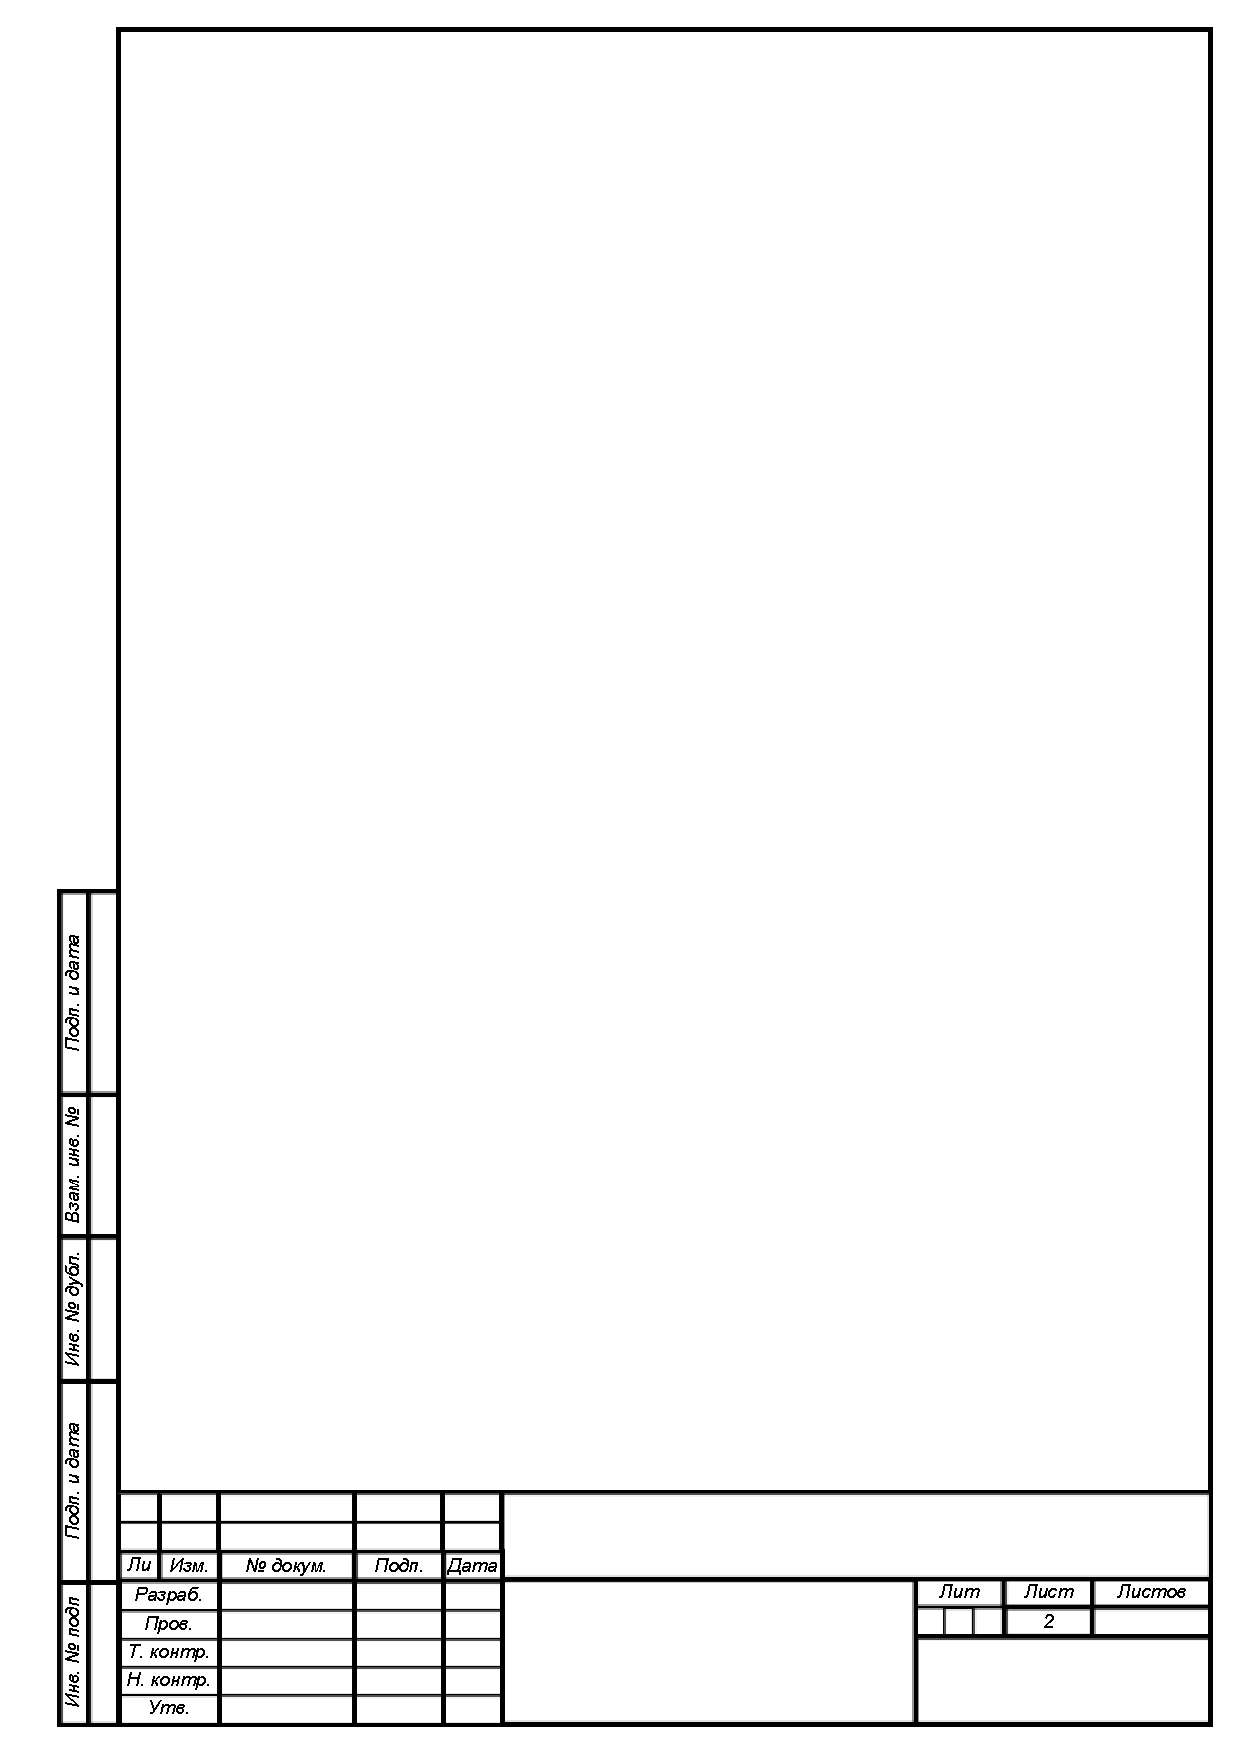
\includegraphics[width=\paperwidth,height=\paperheight]{./myimages/second.pdf}
		\vfill
}}}
		
		
\newcommand\BackgroundPicxx{
	\put(0,0){
		\parbox[b][\paperheight]{\paperwidth}{%
		\vfill
		\centering
		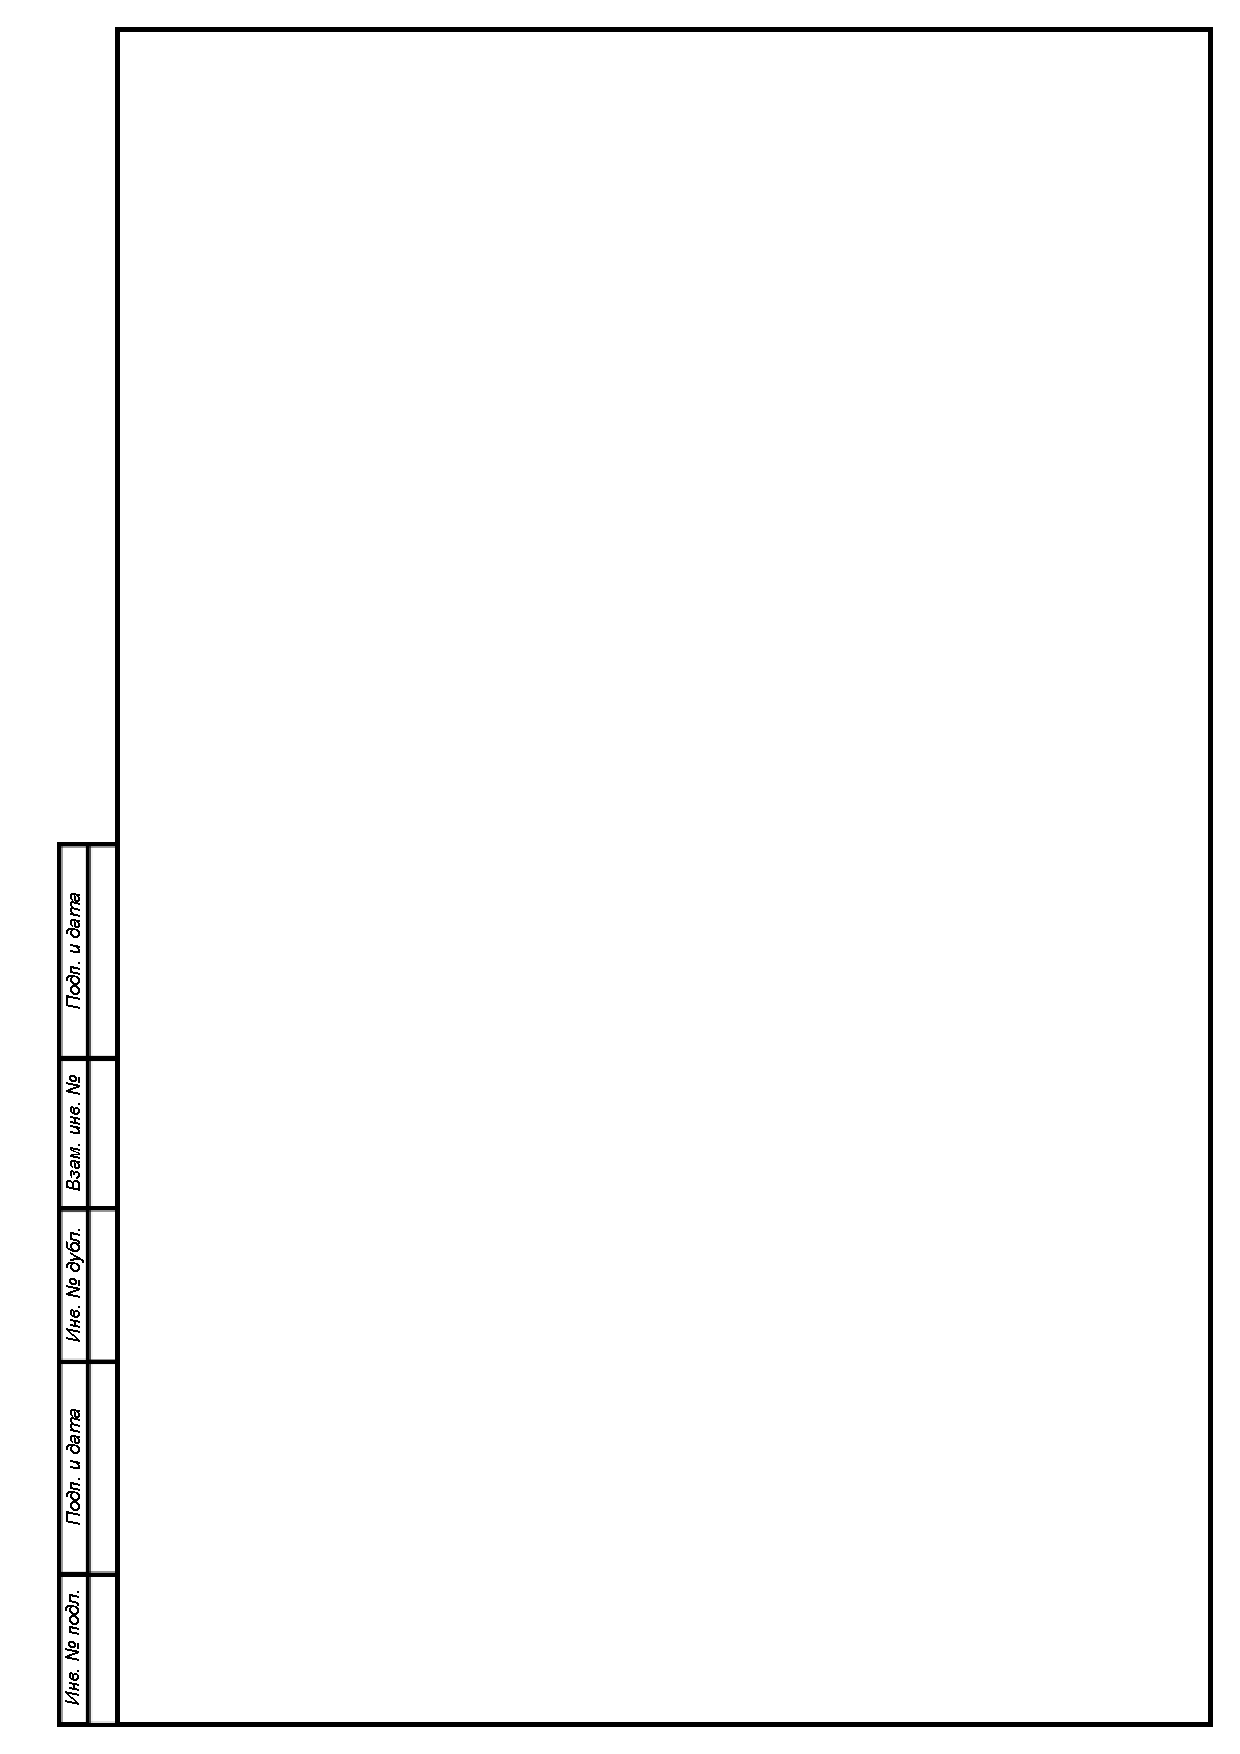
\includegraphics[width=\paperwidth,height=\paperheight]{./myimages/first.pdf}
		\vfill
}}}
				
\newcommand\BackgroundPicx{
	\put(0,0){
		\parbox[b][\paperheight]{\paperwidth}{%
		\vfill
		\centering
		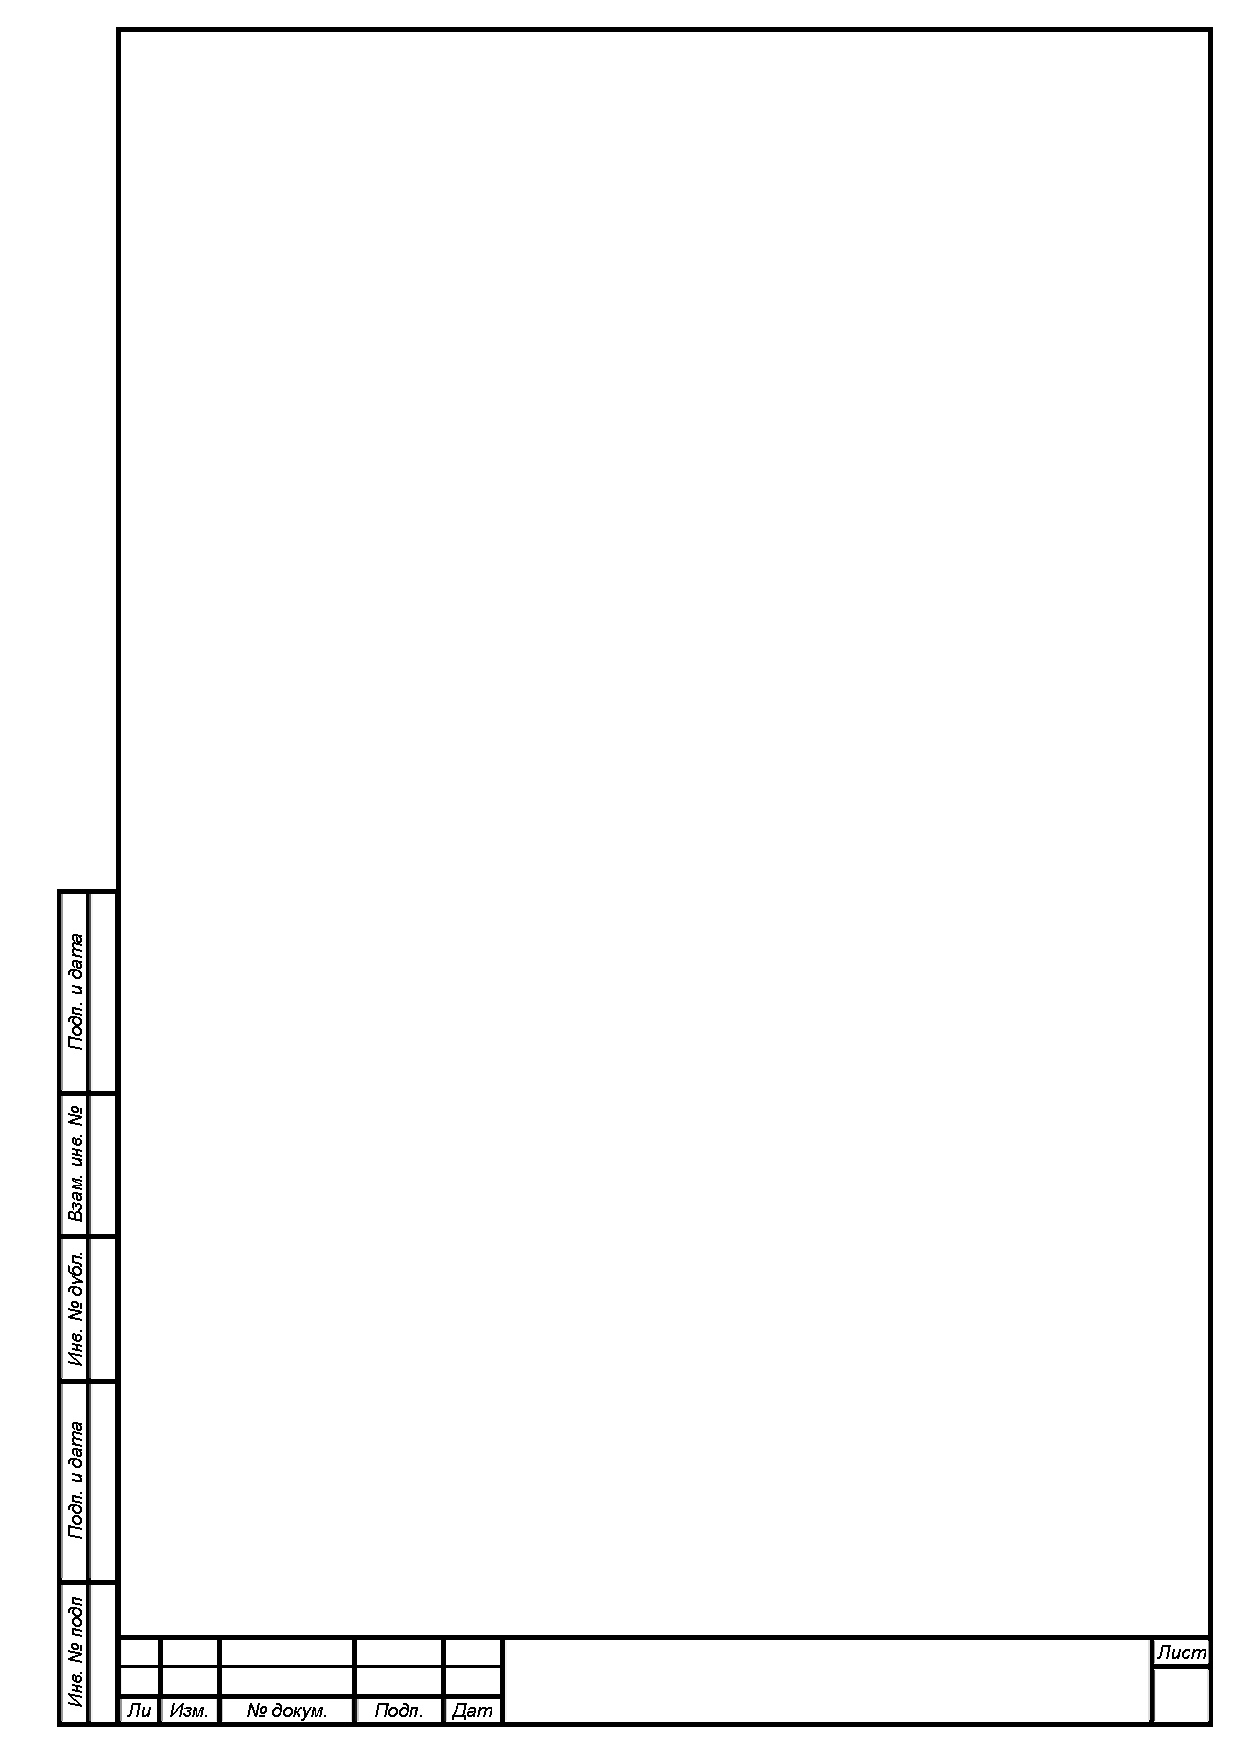
\includegraphics[width=\paperwidth,height=\paperheight]{./myimages/third.pdf}
		\vfill
}}}				
				
\begin{document}
	\AddToShipoutPicture*{\BackgroundPicxx}	
	%%% Переопределение именований %%%
\renewcommand{\abstractname}{Аннотация}
\renewcommand{\alsoname}{см. также}
\renewcommand{\appendixname}{Приложение}
\renewcommand{\bibname}{Литература}
\renewcommand{\ccname}{исх.}
\renewcommand{\chaptername}{}

\renewcommand{\contentsname}{Оглавление}
\renewcommand{\enclname}{вкл.}
\renewcommand{\figurename}{Рисунок}
\renewcommand{\headtoname}{вх.}
\renewcommand{\indexname}{Предметный указатель}
\renewcommand{\listfigurename}{Список рисунков}
\renewcommand{\listtablename}{Список таблиц}
\renewcommand{\pagename}{Стр.}
\renewcommand{\partname}{Часть}
\renewcommand{\refname}{Список литературы}
\renewcommand{\seename}{см.}
\renewcommand{\tablename}{Таблица}

%%% Основные сведения %%%

\newcommand{\thesisSpecialtyNumber}   {\texorpdfstring{{09.04.01}}{XX.XX.XX}}
\newcommand{\thesisSpecialtyTitle}    {\texorpdfstring{{Информатика и вычислительная техника}}{Название специальности}}
\newcommand{\thesisDegree}{{магистра}}
\newcommand{\thesisCity}  {{Нижний Новгород}}
\newcommand{\thesisYear} {{2016}}
\newcommand{\thesisOrganization} {{ФГОУ ВО Нижегородский государственный университет имени~Р.~Е.~Алексеева}}
			% Переопределение именований
	\thispagestyle{empty}%
\begin{center}%
	\MakeUppercase{\thesisOrganization}
\end{center}%
%
\vspace{0pt plus4fill} %число перед fill = кратность относительно некоторого расстояния fill, кусками которого заполнены пустые места
%
\vspace{0pt plus6fill} %число перед fill = кратность относительно некоторого расстояния fill, кусками которого заполнены пустые места
%
\vspace{0pt plus1fill} %число перед fill = кратность относительно некоторого расстояния fill, кусками которого заполнены пустые места
\begin{center}%

\begin{Large}
Лабораторная работа № 1\\
Тема: Программирование калькулятора
	
\end{Large}
	
\end{center}%
%
\vspace{0pt plus5fill} %число перед fill = кратность относительно некоторого расстояния fill, кусками которого заполнены пустые места
\begin{flushright}%
Проверил:\\
Гай В. Е.

Выполнил:\\
Студент гр. 14-В-1\\
Иванов И. И.
\end{flushright}%
%
\vspace{0pt plus4fill} %число перед fill = кратность относительно некоторого расстояния fill, кусками которого заполнены пустые места
\begin{center}%
	{\thesisCity~ \thesisYear}
\end{center}%
\newpage			% Титульный лист
	\AddToShipoutPicture*{\BackgroundPic}	
	\AddToShipoutPicture{\BackgroundPicx}
	\newcommand{\placetextbox}[3]{% \placetextbox{<horizontal pos>}{<vertical pos>}{<stuff>}
	\setbox0=\hbox{#3}% Put <stuff> in a box
	\AddToShipoutPictureFG*{% Add <stuff> to current page foreground
		\put(\LenToUnit{#1\paperwidth},\LenToUnit{#2\paperheight}){\vtop{{\null}\makebox[0pt][c]{#3}}}%
	}%
}%

\pagenumbering{gobble}
\fancyhf{}                          % Очищаем текущие значения

\chapter{Теоретическая часть}						

%\placetextbox{0.55}{0.1}{\Huge \textit{This is my text qweqwqweqw.}}%
%  {<width>}
%  [<left handle>,<top handle>]
%  (<leftmargin>,<topmargin>)

\begin{textblock}{10}[0,0](4.5, 10.9)
	\begin{center}
		\Large	Лабораторная работа № 1\\
	\end{center}
\end{textblock}

\begin{textblock}{4}[0,0](5.5, 11.6)
\begin{center}
\Large	Программирование калькулятора\\
\end{center}
\end{textblock}

\begin{textblock}{3}[0,0](12.5, 11.75)
	\pageref{LastPage}
\end{textblock}

\begin{textblock}{3}[0,0](11, 12.3)
	14-В-1
\end{textblock}
	
	
Способность к звуковому поиску, т.е. определение направления на источник звука – важная вещь для биологических организмов, ведь звук может выступать и сигналом опасности и использоваться для поиска жертвы. К  тому же, локализация звука имеет множество инженерных применений, начиная с определения местоположения говорящего, заканчивая автоматическими решениями куда повернуть направленный микрофон, прожектор или камеру.

В настоящее время актуальна проблема разработки систем оценки направления на источник звука. Такие системы могут использоваться как в масштабах определения местонахождения крупных объектов – например, самолетов, подводных лодок, так и в качестве сенсоров для различных устройств, роботов, охранных систем. 

Во то время, когда задача поиска направления на источник звука приобрела свою актуальность, основное внимание было уделено бинауральному методу поиска, как наиболее очевидному и простому. Этот метод основан на нахождении разницы фаз и величины разности амплитуд между записями с двух приемников звука, находящихся в одной плоскости. Однако, не смотря на работоспособность, такой способ имеет ряд недостатков, среди которых малая область поиска, довольно грубый результат и относительно большие габариты установки.

Использование бинаурального метода поиска обуславливалось тем, что человеческий слух и способность воспринимать направление источника звука долгое время присваивались использованию сразу двух ушей. Однако, когда в некоторых экспериментах бинауральный принцип стал недостаточен, начала серьезно изучаться роль ушной раковины в локализации звука. Некоторые эксперименты проводились с источниками звука, лежащими непосредственно на  медиальной вертикальной плоскости и не отклоняющимися куда-либо по горизонтали. Невозможность использования в таких случаях бинаурального метода послужила толчком к усовершенствованию приемника-обработчика и поиску альтернативных методов решения проблемы.

Была сформулирована задача поиска с использованием одного приемника звука. Существующие решения данной задачи, основанные на монауральном принципе, рассмотрены и приняты во внимание . Многие из этих решений обрабатывают сигнал на уровне отсчетов. С другой стороны, известны факты, утверждающие, что, к примеру, механизмы зрительного восприятия человека целостны, при грубо-точном анализе сенсорных данных зрительной системой. В теории активного восприятия (ТАВ) описан метод грубо-точного анализа, который используется при распознавании изображений. 

\chapter{Практическая часть}						

\pagenumbering{arabic}
\setcounter{page}{3}
\rfoot{\thepage}
\fancyfootoffset[L]{-6cm}
\setlength{\footskip}{1.3cm}
\cfoot[EO]{\fontsize{16}{12} \selectfont \textit{Лабораторная работа № 1} }


Способность к звуковому поиску, т.е. определение направления на источник звука – важная вещь для биологических организмов, ведь звук может выступать и сигналом опасности и использоваться для поиска жертвы. К  тому же, локализация звука имеет множество инженерных применений, начиная с определения местоположения говорящего, заканчивая автоматическими решениями куда повернуть направленный микрофон, прожектор или камеру.

В настоящее время актуальна проблема разработки систем оценки направления на источник звука. Такие системы могут использоваться как в масштабах определения местонахождения крупных объектов – например, самолетов, подводных лодок, так и в качестве сенсоров для различных устройств, роботов, охранных систем. 

\begin{figure}[ht] 
	\center
	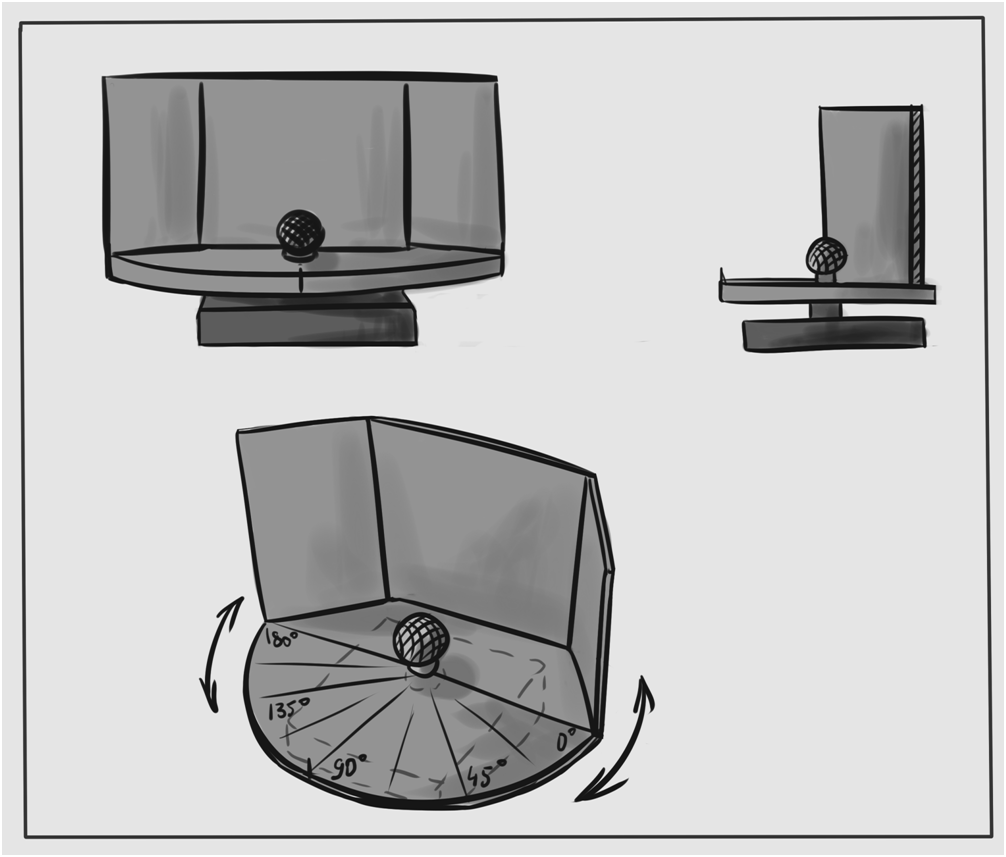
\includegraphics [scale=0.4] {./myimages/pictMaket}
	\caption{Макет установки №1.} 
	\label{img:pictMaket}  
\end{figure}

Во то время, когда задача поиска направления на источник звука приобрела свою актуальность, основное внимание было уделено бинауральному методу поиска, как наиболее очевидному и простому. Этот метод основан на нахождении разницы фаз и величины разности амплитуд между записями с двух приемников звука, находящихся в одной плоскости. Однако, не смотря на работоспособность, такой способ имеет ряд недостатков, среди которых малая область поиска, довольно грубый результат и относительно большие габариты установки.

Использование бинаурального метода поиска обуславливалось тем, что человеческий слух и способность воспринимать направление источника звука долгое время присваивались использованию сразу двух ушей. Однако, когда в некоторых экспериментах бинауральный принцип стал недостаточен, начала серьезно изучаться роль ушной раковины в локализации звука. Некоторые эксперименты проводились с источниками звука, лежащими непосредственно на  медиальной вертикальной плоскости и не отклоняющимися куда-либо по горизонтали. Невозможность использования в таких случаях бинаурального метода послужила толчком к усовершенствованию приемника-обработчика и поиску альтернативных методов решения проблемы.
	% Введение
	\chapter*{Заключение}						% Заголовок
\addcontentsline{toc}{chapter}{Заключение}	% Добавляем его в оглавление

Основные результаты работы заключаются в следующем.
\begin{enumerate}
	
	\item В данной работе был представлен и обоснован пример разработки моделей монауральной локализации источника звука. Предварительно проведен анализ исследований и результатов работы существующих систем, выполняющих схожие задачи.
	
	\item В диссертации исследованы следующие задачи
	
	\begin{enumerate}
		\item Разработана система локализации источника звука, было выполнено построение ее модели и решение с помощью необходимых методов.
		\item Разработана программная реализация модели системы
		\item Выполнено тестирование, включающее в себя проведение экспериментов с реализованной моделью, поиск алгоритма ее работы, дающего наилучший результат, а так же сравнение конечных результатов с аналогами.\\
	\end{enumerate}
	
	  \item В работе адаптирована теория активного восприятия, применительно к обработке и анализу звуковых сигналов
	  
	  \item Все представленные в работе методы реализованы в виде программного обеспечения, способного работать на большом количестве распространенных персональных вычислительных машин.
	  
	  \item По результатам исследований опубликовано несколько статей.
	  
  
\end{enumerate}
В результате выполнения работы были получены знания в областях исследований, имеющих непосредственное отношение к теме магистерской работы: машинном обучении, анализу сигналов, математическом моделировании, улучшены практические навыки разработки программного обеспечения. Получен опыт обоснованного выбора и использования программных продуктов для решения поставленных задач, самостоятельного изучения новых методов исследований и проведения научных исследований в соответствии с тематикой задания. На практике выполнена разработка программной системы, решающей поставленную задачу, а так же проведено ее тестирование с анализом полученных результатов и их сравнением с результатами известных исследований в данной области. Обозначены перспективы дальнейшего модифицирования и развития и системы. 

\clearpage		% Заключение
\end{document}